

\chapter{Determining oceanographic association, movements and connectivity of swordfish in the North Atlantic by integrating electronic tagging and fisheries data}
\label{chap:4}
\raggedbottom
 
%\textbf{Camrin D. Braun\textsuperscript{1,2}*, Peter
%Gaube\textsuperscript{3}, Pedro Afonso\textsuperscript{4,5}, Jorges
%Fontes\textsuperscript{4,5}, Gregory B. Skomal\textsuperscript{6}, Simon
%R. Thorrold\textsuperscript{2}}

%\begin{enumerate}
%\def\labelenumi{\arabic{enumi}.}
%\tightlist
%\item
%  Massachusetts Institute of Technology-Woods Hole Oceanographic
%  Institution Joint Program in Oceanography/Applied Ocean Science and
%  Engineering, Cambridge, MA 02139, USA
%\item
%  Biology Department, Woods Hole Oceanographic Institution, Woods Hole,
%  MA 02543, USA
%\item
%  Air-Sea Interaction and Remote Sensing Department, Applied Physics
%  Laboratory - University of Washington, Seattle, WA, USA
%\item
%  Department of Oceanography and Fisheries, MARE - Marine and
%  Environmental Sciences Centre, University of the Azores, Rua
%  Prof.$\sim$Dr.$\sim$Frederico Machado, Horta, Azores, Portugal
%\item
%  Department of Oceanography and Fisheries, Centre of IMAR of the
%  University of the Azores, Horta, Azores, Portugal
%\item
%  Massachusetts Division of Marine Fisheries, 836 South Rodney French
%  Blvd., New Bedford, MA 02744, USA
%\end{enumerate}

%* Correspondence author. Email:
%\href{mailto:cbraun@whoi.edu}{\nolinkurl{cbraun@whoi.edu}}


{\let\thefootnote\relax\footnotetext{The data used in this study is a collaborative effort among the follow co-authors: C.D. Braun, P. Gaube, P. Afonso, J. Fontes, G.B. Skomal, and S.R. Thorrold}}
%\end{singlespace}
{\let\thefootnote\relax\footnotetext{All authors designed the study. G.B.S., P.A and J.F. conducted the tagging. C.D.B. performed the analysis with P.G. and S.R.T. C.D.B. wrote the paper with contributions and final approval from all authors.}}
{\let\thefootnote\relax\footnotetext{The supplemental methods, figures, and tables for this chapter can be found in Appendix \ref{sec:app4}.}}


\clearpage

\section{Abstract} 

Broadbill swordfish (\textit{Xiphias gladius}) form the basis of commercial fisheries throughout the world's tropical and temperate oceans. Atlantic Ocean swordfish stocks appear to be recovering from years of overfishing, but other populations remain under significant fishing pressure. Management efforts for wide-ranging pelagic fishes, including swordfish, continue to be hindered by data gaps in the basic biology of exploited species. We addressed a significant knowledge gap in the movement ecology of Atlantic swordfish by deploying 20 pop-up satellite archival transmitting (PSAT) tags on individuals captured in the Azores and the Northwest Atlantic (NWA). Reporting tags transmitted low quality light and SST data, so we applied a recently developed geolocation approach that uses hydrographic profile data to improve geolocation accuracy. Resulting tracks from 17 individuals averaged 3,751 km (range 345-7,247) over 93 days (range 17-181). Fish tagged in the Azores primarily moved between the Azores archipelago and the Azores Front south of the islands. Movements of fish tagged in the NWA spanned 35$^\circ$ of latitude from summer foraging grounds near the Grand Banks to winter habitats near the Antillean Arc. We also mined fisheries-dependent data from the International Commission for the Conservation of Atlantic Tunas (ICCAT) databases. We used ICCAT data from 15,101 conventional tag releases and 568 recaptures, as well as catch-per-unit effort (CPUE) data from $\sim$135 million and 1.7 billion hooks set by the U.S. and international longline fleets, respectively, to supplement the satellite tag data. Movements and displacement of satellite and conventional tags indicated complex stock structure within the North Atlantic. Across all three datasets, swordfish exhibited remarkable physiological capabilities by occupying a $\sim$25$^\circ$C SST range in primarily oligotrophic waters and frequented active front boundaries. These data also suggested swordfish occupied eddies across the study region and satellite- and conventional-tagging data suggest a possible preference for anticyclones, although the influence of fishing effort cannot be ruled out. Generalized additive modeling corroborated the eddy results and also highlighted the importance of geographic location influencing CPUE, as well as SST, chlorophyll and minor contributions from other predictor variables. Our work demonstrates the utility in synthesizing results from fishery-independent electronic tag data and fisheries datasets to improve understanding of oceanographic influences on swordfish.

\section{Introduction}%\label{introduction}

Swordfish have the broadest geographical distribution of all billfishes \citep{Braun2015} and are found worldwide from 45$^{\circ}$S to 45$^{\circ}$N \citep{Palko1981}. This species is the target of the most valuable and ubiquitous commercial billfish fishery in the world \citep{FAO2012} which has historically led to the overexploitation of swordfish stocks. Despite their economic value, swordfish now appear to be adequately managed throughout the Atlantic, with North Atlantic stocks exhibiting recovery after years of overfishing \citep{Neilson2013, Collette2011}. The Atlantic swordfish population is currently managed as three stocks (North, South and Mediterranean) based on conventional \citep{Garcia-Cortes2003} and satellite \citep{Neilson2009, Abascal2015} tagging and analyses of population genetics \citep{Bremer1996, AlvaradoBremer2005a, Smith2015}. However, recent genetic evidence suggests that the boundary between north and south stocks may require revision \citep{Smith2015}, and some tagging studies have observed potential structure within the North Atlantic \citep{Neilson2009, Abascal2015}.

Most of the existing research on Atlantic swordfish is driven by stock assessment needs. Nearly all biological and ecological parameters are derived from the relatively extensive work in the NWA compared to the rest of the Atlantic basin. Tagging studies indicate North Atlantic swordfish exhibit largely North-South movements driven by contrasting ocean regimes for feeding and reproduction \citep{Sedberry2001, Neilson2009, Abascal2015} in which they move from productive foraging grounds in the far north during summer to warm tropical and subtropical waters in winter to spawn and to promote larval growth \citep{Arocha1995}. During these movements, they exhibit extreme physiological versatility in which they regularly experience a 15$^{\circ}$C daily temperature range \citep{Abascal2015} during regular diel vertical migrations \citep{Carey1981, Lerner2013} to the deep scattering layer \citep{Carey1990a, Josse1998}. 

Reliable stock assessments, including habitat-based vulnerability models and CPUE corrections \citep{Hinton1996, Bigelow2007}, and detecting effects of climate changes \citep{Schirripa2016} rely on a thorough understanding of the oceanographic characteristics driving animal behavior. For instance, physical-biological interactions that occur at the oceanic mesoscale \citep[$\mathcal{O}$(10-100 km);][]{McGillicuddy2016} and submesoscale \citep[$\mathcal{O}$(1 km); ][]{flierl2002mesoscale, levy2012bringing} are known to influence pelagic fishes \citep{teo2010comparative, Seki2002, godo2012mesoscale}, including swordfish \citep{Podesta1993, Scales2017}. Eddies, currents and fronts are the main features that occur at these scales and influence animal movements \citep{Hobday2014}. These features play a fundamental role in ocean dynamics, by structuring the physical and biological properties of the marine environment, and remain important foci for current physical-biological interactions research today \citep{McGillicuddy2016}.

The influence of oceanography on swordfish abundance and behavior has been investigated for decades, but these approaches have relied heavily on fisheries-dependent CPUE data and have yielded conflicting results. For example, \citet{Podesta1993} determined high swordfish CPUE more frequently occurred in the vicinity of fronts but showed no statistical relationship with frontal density or SST gradient, whereas \citet{Bigelow1999} found a positive relationship between swordfish CPUE and several front metrics. In addition, while > 90 satellite archival tags have been deployed on swordfish in the North Atlantic \citep{Braun2015}, geolocation error has largely precluded quantitative analyses of horizontal movements in the context of oceanography. As such, oceanographic drivers of swordfish movements remain poorly understood. Here, we analyze a fisheries-independent satellite tagging program on swordfish in the North Atlantic. We then combine high-resolution satellite tag data with inference from > 15,000 conventional tag deployments and CPUE data from nearly 2 billion longline hooks to synthesize oceanographic drivers, movements and connectivity of swordfish in the North Atlantic.

\section{Materials and methods}

\subsection{Satellite tagging}\label{sat-tag-methods}

We deployed 20 pop-up satellite archival transmitting (PSAT) tags (17 miniPAT, 3 MK10-AF; Wildlife Computers Inc., Redmond, WA, USA) on swordfish (\textit{Xiphias gladius}) in the North Atlantic between 2009-2014, including 8 near the Grand Banks, 5 in the southern Sargasso Sea and 7 around the Azores (Table \ref{tab:tagtable}). Tags logged depth, temperature, and light level data every 10 seconds (Mk10-AF) or 15 seconds (miniPAT) to onboard memory. All tags recorded light data for geolocation purposes, and the Mk10-AF tags housed a Fastloc GPS receiver for acquiring high-resolution location information. Swordfish in the Azores were caught on rod and reel and brought alongside or onto the tagging vessel for tag placement. NWA swordfish were caught by a commercial longline vessel, brought alongside the boat and tagged if judged to be in good condition by the vessel captain. Weight and lower jaw fork length (LJFL) were estimated by the tagging team. Tags were applied into the dorsal musculature near the base of the dorsal fin using a titanium plate or nylon umbrella dart as an anchor. Tags were released from the swordfish using a corrosive burn wire at pre-programmed dates during tag deployment (range of programmed deployment duration 90-181 days). After the tags released and floated to the surface, summarized data were transmitted to Argos satellites until battery failure. Transmitted data were decoded with manufacturer software (WC-DAP 3.0, Wildlife Computers, Inc., Redmond, WA). All data from tags that released prematurely after less than 10 days were removed from all analyses. All further analyses were conducted in \texttt{R} \citep{RDevelopmentCoreTeam2015}, and a Kruskal-Wallis test was used to compare density distributions. For visualization purposes, tag-based depth-temperature profile plots were constructed by computing a weighted least-squares regression (LOESS) using half-power cutoffs of $\pm$ 5 days and 150 m from all daily depth-temperature data (\texttt{R} code available on request). This research was performed in accordance with the Woods Hole Oceanographic Institution's Animal Care and Use Committee (IACUC) protocol \#16518.

\subsubsection{Geolocation methods}

Most probable tracks for PSAT-tagged swordfish were constructed using the \texttt{HMMoce} package \citep[][Chp. \ref{chap:2}]{Braun2018a} for \texttt{R} \citep{RDevelopmentCoreTeam2015}. This approach uses light-levels, sea surface temperature, depth-temperature profiles and bathymetry recorded by archival tags, with observations and model outputs, to construct likelihoods of the tagged individual's movements. Likelihoods are convolved in a gridded hidden Markov model that computes posterior probability distributions to estimate the most likely state (position and behavior) of the animal at each time point.

Observation-based likelihoods were derived from remotely-sensed SST, light-based longitude and depth-temperature profile data collected by the tags, using four separate likelihood calculations: \emph{1)} An SST likelihood was generated for tag-based SST values integrated according to an error term (\(\pm\) 1\%) and compared to remotely-sensed SST from daily optimally-interpolated sea surface temperature (OI-SST, 0.25$^{\circ}$ resolution) fields \citep{Reynolds2007, Banzon2016}. \emph{2)} Light-based longitude likelihood was derived using estimates of longitude from GPE2 software (Wildlife Computers, Inc.) that facilitated visual checking of light curves. \emph{3)} Depth-temperature profiles recorded by the tag were compared to daily reanalysis model depth-temperature products from the HYbrid Coordinate Ocean Model \citep[HYCOM, 0.08$^{\circ}$ resolution;][]{Bleck2002, Chassignet2007} at standard depth levels available in these products. Individual likelihood surfaces for each depth level were then multiplied together for an overall profile likelihood at that time point. \emph{4)} Ocean Heat Content (OHC) was obtained by integrating the heat content of the water column above the minimum daily temperature to the most shallow depth recorded by the tag for both the tag profiles and HYCOM fields \citep{Luo2015, Braun2018a}. Start and end locations were considered known in all cases and model runs.

The resulting observation likelihoods, in all possible pairwise and triplicate combinations, were convolved with two different movement kernels representing resident and migratory behavior "states" of tagged fish. For full details of the convolution, filtering and smoothing components of the model see \citet{Braun2018a} (Chapter \ref{chap:2}). Parameter estimation was performed using an Expectation-Maximization algorithm following \citet{Woillez2016}, and model selection used Akaike Information Criterion (AIC). Results from the final smoothing step of the selected model represent the posterior distribution of each state over time. Distributions were summed for each behavior state and time step to determine the most likely behavior state at each time. The mean of the daily distributions was used to calculate a most probable track.

%--------------------
\clearpage
\begin{landscape}
\begin{table}
\caption[Summary of swordfish tagged with PSATs in the North Atlantic Ocean]{Summary of swordfish tagged with PSATs in the North Atlantic Ocean. Est Wt = Estimated weight (kgs). Stage = stage of maturity for juvenile (J), sub-adult (SA) and adult (A) swordfish. Tag types are miniPAT (mP) or FastLOC (fL). Region indicates where an individual was tagged and refers to the Grand Banks (GB), the Azores (AZ) or offshore from Florida in the southern Sargasso Sea (FL). Time-at-liberty (TAL) is in days. Distance (Dist.) is cumulative track distance in km. PDT, Light and SST = percent of deployment period with depth-temperature profiles (PDT), light and sea surface temperature (SST) data, respectively. Observation likelihoods (Obs.) indicate observations used in \texttt{HMMoce} to construct the most probable track: L=light-based longitude, S=sea surface temperature, H=HYCOM depth-temperature profiles, O=integrated Ocean Heat Content, F=Fastloc GPS, DD=data deficient.}
\label{tab:tagtable}
\centering
%\begin{tabular}[t]{rlrrrlllllllllll}
\resizebox{9in}{!}{%
\begin{tabular}{p{1cm} p{2cm} p{1cm} p{1cm} p{1cm} p{0.85cm} p{0.75cm} p{0.85cm} p{1cm} p{1cm} p{1cm} p{1cm} p{1cm} p{1cm} p{1cm} p{1cm}}
\toprule
ID & Tag Date & Tag Lat & Tag Lon & Est Wt & Stage & Type & Region & TAL & Pop Lat & Pop Lon & Dist. & PDT (\%) & Light  (\%) & SST  (\%) & Obs. \\
\midrule
98751 & 2009-12-02 & 38.44 & -28.52 & 11.0 & J & mP & AZ & 17 & 32.92 & -28.18 & 773 & 88 & 47 & 82 & LSH\\
104668 & 2011-10-21 & 38.41 & -28.51 & 19.5 & J & mP & AZ & 35 & 27.17 & -30.92 & 2590 & 91 & 9 & 89 & LSH\\
104670 & 2011-10-21 & 38.44 & -28.56 & 23.5 & J & mP & AZ & 26 & 31.9 & -30.89 & 902 & 88 & 85 & 42 & LSH\\
98721 & 2011-10-26 & 38.44 & -28.54 & 12.0 & J & mP & AZ & 38 & 38.55 & -28.91 & 345 & 95 & 5 & 8 & LSH\\
98722 & 2011-10-26 & 38.43 & -28.53 & 11.0 & J & mP & AZ & 150 & 38.17 & -28.56 & 5335 & 60 & 24 & 81 & LSH\\
104671 & 2011-11-15 & 37.84 & -27.17 & 17.5 & J & mP & AZ & 150 & 37.84 & -27.17 & 4816 & 71 & 33 & 91 & LSH\\
104672 & 2011-11-15 & 37.84 & -27.17 & 10.0 & J & mP & AZ & 55 & 33.54 & -28.53 & 2357 & 96 & 38 & 98 & LSH\\
100976 & 2010-11-25 & 28.20 & -66.92 & 50.0 & SA & mP & FL & 24 & 20.27 & -65.05 & 979 & 92 & 0 & 92 & LH\\
100980 & 2010-11-30 & 28.34 & -67.52 & 68.2 & A & mP & FL & 90 & 30.84 & -75.17 & 3828 & 94 & 1 & 73 & LSH\\
100978 & 2011-01-10 & 27.57 & -67.92 & 45.5 & SA & mP & FL & DD &  &  &  &  &  &  & DD\\
95975 & 2011-01-20 & 24.61 & -68.58 & 56.8 & SA & mP & FL & 181 & 38.93 & -53.2 & 6782 & 83 & 9 & 81 & LSH\\
95983 & 2011-01-31 & 25.90 & -69.53 & 56.8 & SA & mP & FL & DNR &  &  &  &  &  &  & \\
110490 & 2011-09-15 & 43.67 & -48.81 & 81.8 & A & mP & GB & 90 & 30.29 & -63.63 & 4449 & 79 & 39 & 96 & LSH\\
110491 & 2011-09-15 & 43.65 & -48.82 & 81.8 & A & mP & GB & 180 & 12.35 & -60.04 & 6914 & 36 & 33 & 64 & LSH\\
110497 & 2011-09-19 & 43.94 & -48.57 & 65.9 & A & mP & GB & 90 & 18.7 & -76.16 & 4869 & 72 & 21 & 70 & LH\\
110498 & 2011-09-22 & 43.90 & -48.40 & 100.0 & A & mP & GB & 90 & 32.38 & -59.38 & 2718 & 74 & 14 & 83 & LSH\\
110496 & 2011-10-17 & 44.57 & -46.90 & 61.4 & A & mP & GB & 149 & 34.95 & -50.37 & 7247 & 99 & 32 & 97 & LSO\\
106788 & 2013-09-27 & 46.69 & -45.80 & 90.9 & A & fL & GB & 180 & 20 & -74.28 & 6714 & 27 & 1 & 3 & LSH\\
106795 & 2013-09-27 & 46.48 & -45.56 & 90.9 & A & fL & GB & 40 & 31.03 & -39.68 & 2146 & 95 & 28 & 70 & FLSH\\
106797 & 2013-09-27 & 46.62 & -45.64 & 68.2 & A & fL & GB & DNR &  &  &  &  &  &  & \\
\bottomrule
\end{tabular}}
\end{table}
\end{landscape}
\clearpage
%--------------------

\subsection{Fisheries data}%\label{fisheries-data}

To evaluate movements of satellite-tagged fish in relation to the swordfish longline fishery in the North Atlantic, we obtained fisheries data (Task II catch--effort; version Nov. 2016) from the ICCAT Secretariat \href{http://www.iccat.int/en/accesingdb.htm}{(http://www.iccat.int/en/accesingdb.htm)}. We extracted longline (LL) data for the years 1990-2010 in the North Atlantic west of 20$^{\circ}$W at two different spatial resolutions: 1) 1$^{\circ}$ x 1$^{\circ}$ for the U.S. fleet and 2) 5$^{\circ}$ x 5$^{\circ}$ resolution data available for the international fleets from Brazil, China, Cuba, Greece, Japan, Korea, Libya, Mexico, Spain, U.K., Uruguay. Longline catch data were used to calculate mean catch per unit effort (CPUE; number of fish per 1000 hooks) in each grid cell. CPUE data resulting in > 200 fish per 1000 hooks were considered an error and removed from the dataset. We also obtained conventional tag data from the ICCAT Secretariat tag database for swordfish in the North Atlantic from 1940-2016.

\subsection{Oceanographic data}

In order to characterize associations between swordfish and the
oceanographic environment, we acquired remote sensing and climatological data from multiple sources. We used a monthly composite of remotely-sensed Chlorophyll-a from SeaWiFS (nominal resolution of 9 km) and bathymetry from Smith and Sandwell (0.0167$^{\circ}$ resolution, version 11.1). Distance to the 200 m bottom contour was calculated from bathymetry. Daily sea surface temperature (SST) data were acquired from the HYCOM reanalysis product (global 0.08$^{\circ}$ daily resolution) due to the broad temporal coverage of the swordfish data. Although the HYCOM data were modeled SST, these data were comparable to remotely-sensed SST from Multi-scale Ultra-high Resolution (MUR) data (global 0.01$^{\circ}$ daily resolution) during the shorter period in which both were available (Fig. \ref{fig:a4f1}). Fronts were detected in daily HYCOM SST fields using a threshold algorithm \citep{Belkin2009} implemented in the \texttt{boaR} package \citep{Galuardi2017} for \texttt{R} and composited to monthly front frequency using thermal front magnitude >0.1$^{\circ}$C $\cdot$ km$^{-1}$. We used monthly global estimates of climatological isothermal ($\Delta T$=0.2$^{\circ}$C) mixed layer depth \citep{DeBoyerMontegut2004}, and a climatological representation of the north wall of the Gulf Stream defined as the position of the 15$^{\circ}$C contour at 200 m in climatological annual mean temperature from the World Ocean Atlas (2013, 0.25$^{\circ}$ global) \citep{Fuglister1963, Gaube2017DSR}.

Monthly mean sea surface height (SSH, global 0.25$^{\circ}$) was computed from AVISO sea-level anomaly (SLA) data by removing the result of high-pass filtering the SLA fields using a 20$^\circ$x10$^\circ$ (lon x lat) 2D LOESS smoother to remove effects of seasonal heating and cooling \citep{Chelton2011} as:

\begin{equation}
SSH = SLA - \left<SLA\right>
\end{equation}

where the $<>$ operator indicates spatial smoothing. We derived a monthly climatology for deep scattering layer depth (\(Z_{DSL}\)) based on a stepwise multiple linear regression from \citet{Bianchi2013}:

\begin{equation}
Z_{DSL} = 398 - 0.56 \cdot \Delta O_2 - 115 \cdot Log(CHL) + 0.36 \cdot MLD - 2.4 \cdot \Delta T
\label{eq:dsl}
\end{equation}

where \(\Delta O_2\) and \(\Delta T\) were differences between 0-25 m and 150-500 m in monthly climatological mean oxygen and temperature data, respectively, from the World Ocean Atlas 2013 \citep{Garcia2013, Locarnini2013}. Finally, we used the monthly composite of chlorophyll data (\(CHL\)) from SeaWiFS and the mixed layer depth climatology described above (\(MLD\)).

To quantify associations between swordfish and mesoscale eddies, we collocated conventional tag data to the Mesoscale Eddy Trajectory Atlas from Aviso that contains daily tracks of coherent mesoscale structures (CMS) based on maps of sea surface height \citep{Chelton2011}. We developed a meander filter \citep[similar to][]{Gaube2017DSR} for the Gulf Stream and Gulf of Mexico region in which we defined a mask \(\pm\) 1$^{\circ}$ north and south from the 40 cm ADT contour that approximated the north wall of the Gulf Stream and the Loop Current in the Gulf of Mexico to distinguish between mesoscale eddies and meanders. The mask was extended to 2$^{\circ}$ south of the ADT contour in the Gulf Stream to eliminate anticyclonic meanders. Those features in which the core of the CMS was within the meander mask were considered meanders and removed from the remainder of the analysis.

We visually compared swordfish tracks and depth-temperature profile data from the PSAT tags to the SSH fields and tracked eddies to generate a qualitative comparison of eddy use from these data. Eddy occupation was quantified using a subset of the conventional tag data to include those swordfish release and recapture positions that were in regions of known mesoscale activity, including the Gulf Stream, Sargasso Sea and Gulf of Mexico, in water deeper than 2000 m and that corresponded to the temporal limits of the eddy tracking dataset (Jan 1993 - Sept 2016). These locations were collocated to the nearest eddy identified in the eddy atlas, after applying the meander filter in the Gulf Stream and Gulf of Mexico. To assess differences in the distribution of swordfish in anticyclonic and cyclonic eddies, we constructed histograms of swordfish location as a function of normalized radial distance ($r$), defined as the geographic distance ($d$) normalized by the speed-based eddy radius scale $L_s$.  The resulting histogram values were then normalized by the area of each radial annulus defined by the histogram bin size and the distance $r$ from the eddy center. To determine if swordfish were more likely to be associated with the core, interior or periphery of eddies of either polarity, we defined eddy subregions by the normalized distance ($r$) from the eddy SSH extremum, where the inner-core is defined as $r \leq L_s/2$, the outer core as $L_s/2 < r \leq L_s$ and the eddy interior includes both the inner and outer core $r \leq L_s$. The eddy periphery is defined as $L_s < r \leq 2L_s$ and the area outside of an eddy as $r > 2L_s$ \citep[see Fig. 2 in][]{Gaube2017}. To assess the role of passive advection and the relative spatial composition of the sub-regions of eddies of each polarity, we also collocated a surface drifter dataset. The drifter dataset was acquired from NOAA's Atlantic Oceanographic and Meteorological Laboratory, and we used all drifters within each study region for a 5-year period (2005-2009) (Fig. \ref{fig:a4f2}).

\subsection{GAM model formulation}

Oceanographic variables were used to develop generalized additive models (GAMs) to quantify the relationship between the physical environment and swordfish CPUE from the U.S. longline fleet. The oceanographic variables considered in model development were: SST ($^{\circ}$C), SSH (m), chlorophyll-a (\(mg \cdot m^{-3}\)), climatological DSL depth (m), climatological MLD (m), thermal front range ($^{\circ}$C) and frequency (days \(\cdot\) month\(^{-1}\)), bottom depth (m), distance to climatological position of the Gulf Stream (km) and distance to the 200 m depth contour. Due to the summarized nature of the catch data (monthly, 1$^{\circ}$ grid), oceanographic variables were all summarized as necessary to match this spatial and temporal scale. Front range was collinear with SST and removed. Bathymetry was collinear with the distance to the 200 m contour so standard deviation of bathymetry within a grid cell was used instead. Zero values were removed from the CPUE data to avoid zero-inflation in the model \citep{Zuur2009, Maunder2004}, effectively allowing us to model oceanographic drivers of varying catch (rather than presence-absence).

GAMs were constructed with the \texttt{mgcv} package \citep{Wood2006} in \texttt{R} using the negative binomial family with a log-link function. Explanatory variables (except month) were modeled as continuous and smoothed by functions chosen automatically using the \texttt{mgcv} package and checked manually. The base model, after adjusting for collinearity, included 12 predictor variables for which the model was formulated as:

\begin{equation}
CPUE = S(Location) + Month + f_1(X_1) + f_2(X_2) + ... + f_j(X_j)
\label{eq:gam}
\end{equation}

where \(S\) is a smoothing function for location (longitude, latitude); \(f_1...f_j\) are smoothing functions for environmental variable 1:\(j\); \(X_1...X_j\) are values of the environmental variable \(j\). Each smoothing function, with the exception of location, was permitted three degrees of freedom to minimize overfitting \citep{Rooker2012}. A stepwise backwards selection approach using Akaike Information Criterion (AIC) was used to select the final model. Predictor variables that were statistically significant at \(p \leq\) 0.05 were retained during selection and models were evaluated by checking diagnostic plots on fitted data and residuals (Fig. \ref{fig:a4f3}).

%--------------------
\begin{figure}[htbp]
\centering
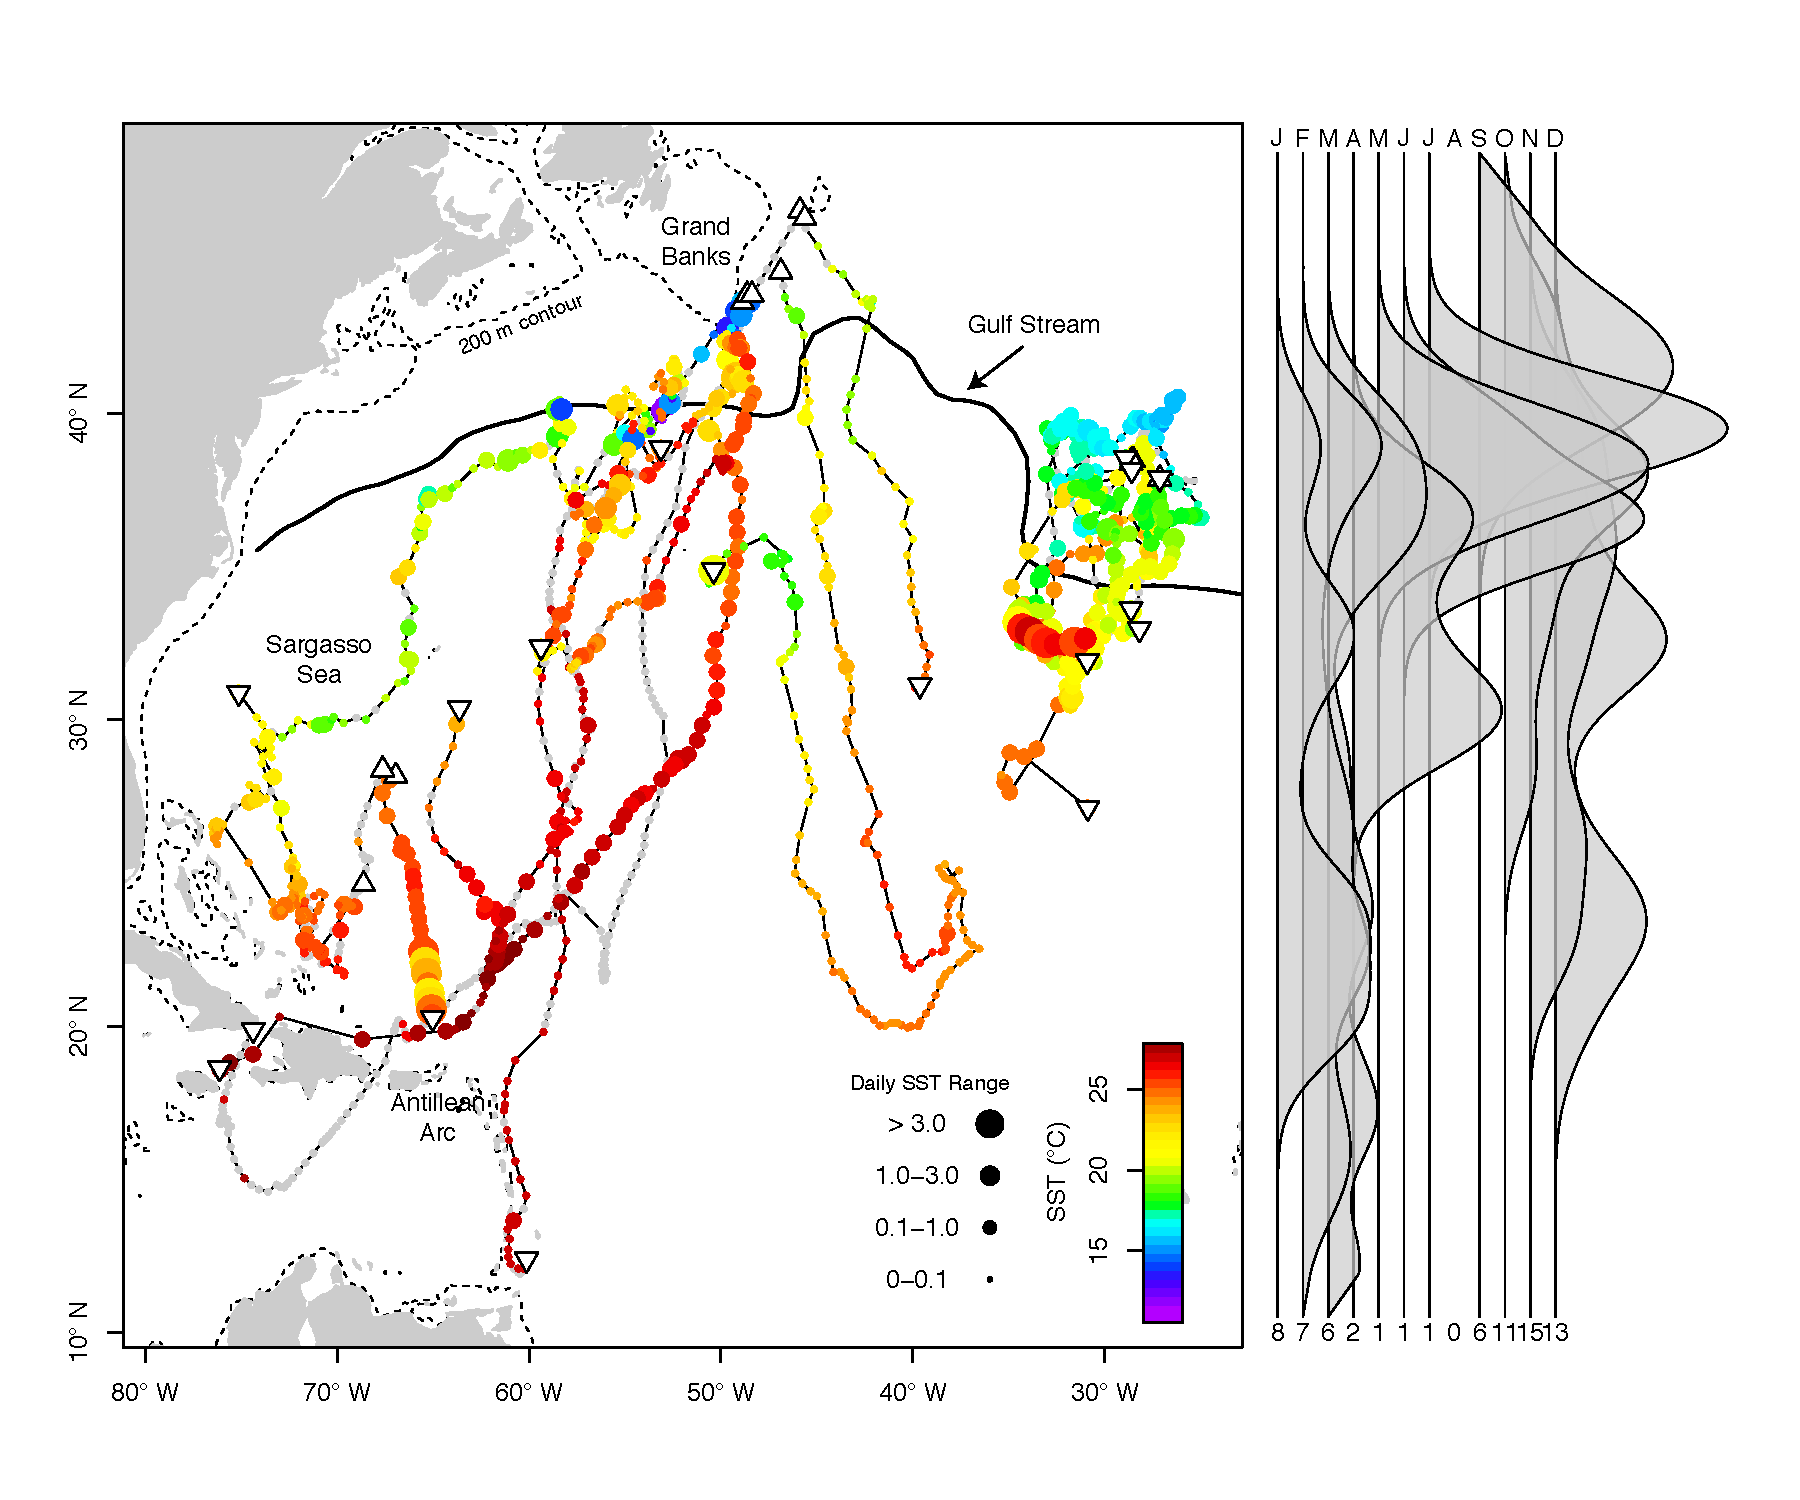
\includegraphics[width=\textwidth]{images/C4_Fig1.pdf}
\caption[Movements of satellite-tagged swordfish in the North Atlantic]{Movements of satellite-tagged swordfish in the North Atlantic. Most probable track estimates (left panel) for swordfish in which point color indicates tag-measured sea surface temperature (SST), and point size indicates the range of daily SST measured. Upward and downward pointing triangles represent release and pop-up positions, respectively. Dashed point and line contours represent the mean Gulf Stream position (see methods) and the 200m bathymetric contour, respectively. Right panel shows monthly density distribution of satellite-tagged swordfish by latitude. Upper letters indicate month and lower number labels indicate sample size of tagged individuals.}
\label{fig:c4f1}
\end{figure}
%--------------------

\section{Results}

Seventeen of the 20 PSAT tags deployed in this study reported and transmitted data, 9 of which were shed prematurely. The 17 reporting tags were at liberty for an average 93 days (range 17-181), and one tag was physically recovered after 149 days at liberty (PTT 110496; Table \ref{tab:tagtable}). All individuals (n=7) tagged near the Azores were juveniles with a mean estimated weight of 15 kgs (range 10-24 kgs). The largest individuals were adults tagged near the Grand Banks (n=8) which averaged 80 kgs (range 61-100 kgs), and those tagged in the western Atlantic were a mix of adult (n=1) and subadult (n=4) fish averaging 55 kgs (range 46-68 kgs).

The conventional tag database contained 15,101 swordfish releases and 568 recaptures from 1940 to 2016. The ICCAT Task II database contained catch and effort data from $\sim$135 million hooks set by the US longline fleet from 1990-2009 gridded at 1$^{\circ}$ spatial resolution. This effort resulted in catch of 1.2 million swordfish with a mean CPUE of 12 fish / 1000 hooks (range 0-200). Data were available for longline vessels from other flag countries that set $\sim$1.7 billion hooks in the North Atlantic from 1990-2009. Approximately 4 million swordfish were harvested during this time period with mean CPUE of 3.4 fish / 1000 hooks (range 0-72). Most of the reported non-US catch data came from the Japanese (52\%), Chinese (23\%) and Spanish (22\%) fleets.

\subsection{Geolocation of PSATs}%\label{geolocation-of-psats}

Varying amounts of each data type were obtained from the PSATs for estimating most probable tracks (Table \ref{tab:tagtable}). Sufficient light available for geolocation was generally low (mean 25\% of deployment days, range 0-85\%). SST and depth-temperature profile (PDT) data were recorded for a higher percentage of deployment days than light data in all but one transmitted dataset, and on average comprised 72\% and 79\% of deployment days respectively (range 3-98\% for SST and range 27-99\% for PDT). Two (out of 3 deployed) Fastloc tags reported data, but only one (PTT 106795) reported two realistic GPS positions collected during the deployment.

\subsection{Horizontal movements}%\label{horizontal-movements}

Overall movements of PSAT-tagged swordfish ranged from 345 to 7,247 km in up to 181 days at liberty and were predominantly oriented north-south (Fig. \ref{fig:c4f1}). We found no significant relationship between fish size and displacement using linear regression, and we found no significant difference in movement rates among fish from the three different tagging regions. The PSAT-tagged adults in the NWA moved across a 35$^{\circ}$ latitudinal range between temperate waters in the summer as far north as the Grand Banks and tropical or subtropical waters during winter from the Caribbean to coastal Florida (10-30$^{\circ}$N)(Fig. \ref{fig:c4f1}). Model selection favored HYCOM-based profile likelihoods in 16 of 17 track calculations. The remaining geolocation analysis leveraged OHC-based profile likelihoods to generate the most likely track estimate (Table \ref{tab:tagtable}). State-switching dynamics in \texttt{HMMoce} suggested the migratory behavior state occurred 3 times more often than did residency behavior (not shown) and dominated as individuals traversed the Sargasso Sea or while the individuals tagged in the Azores moved through the southern extent of the observed movements. In contrast, more tortuous, resident-like behavior was common along the Antillean Arc, the Azores archipelago and in the "loop" movement exhibited around 20$^{\circ}$N and 40$^{\circ}$W along the mid-Atlantic Ridge by an adult tagged on the Grand Banks (Fig. \ref{fig:c4f1}). These habitats were connected by long-range, relatively directed movements through the Sargasso Sea with the majority of more tortuous movements occurring in the Gulf Stream and from the Bahamas southeast along the Antillean Arc and southern Sargasso Sea (range of cumulative track distances 979-7,247 km).

Seven tags were deployed on adults near the Grand Banks in September and October, and, by mid-October, all had left the tagging region. In early November, six individuals had crossed the Gulf Stream moving southwest into tropical water ($\sim$28-30$^{\circ}$C) south of 30$^{\circ}$N by December. The remaining individual tagged on the Grand Banks (PTT 110491) moved into the Gulf Stream in early November and remained mostly along the north wall until late December. Overwintering habitat was centered around 20$^{\circ}$N but spanned 30$^{\circ}$ of longitude from the eastern Caribbean and the NE coast of Venezuela to as far east as the mid-Atlantic Ridge. The individual tagged on the Grand Banks that moved SE to the mid-Atlantic Ridge began a return migration to the north in mid-February, but this tag popped up prematurely in mid-March along the 20$^{\circ}$C isotherm near 35$^{\circ}$N. A single tag from January deployments off Florida transmitted reliable data (PTT 95975). This dataset comprised the only spring movements observed in this study and indicated northward migration began around mid-April arriving to the Gulf Stream by May where this fish remained through mid-July.

The juveniles and subadults tagged near the Azores exhibited relatively restricted movements, in both latitudinal range (27-40$^{\circ}$N) and overall distance (345-5,335 km), as compared to the larger fish tagged in the NWA. These individuals were tagged in late October and early November around 38$^{\circ}$N and, in general, moved south into the warmer, Azores Front region at $\sim$32$^{\circ}$N. Of the 3 tags at liberty in January, 1 returned to the Azores in late December followed by a second that returned in mid-February. The third tag deployment ended in early January at 33$^{\circ}$S.

Seasonality observed in both conventional tag and catch data was similar to the movements by the satellite-tagged fish (Fig. \ref{fig:a4f4}). In general, CPUE was highest along the Grand Banks, the central North Atlantic and around Bermuda in the summer and moved away from northern latitudes in the winter (Fig. \ref{fig:c4f2}). During winter and spring months, CPUE was focused from the Gulf of Mexico, east to the southeastern U.S., Caribbean Sea, and along the Antilles. Effort began returning north, particularly by the international (non-U.S.) fleet, in spring and most longline fishing effort returned northward to the Grand Banks and extended south to $\sim$20$^{\circ}$N in the central North Atlantic by summer (Fig. \ref{fig:c4f2}). The majority of conventional tags were deployed and recovered along the eastern seaboard of the U.S. but spanned the North Atlantic from the Gulf coast of Texas to Europe and from the Amazon Delta to the Grand Banks. Conventional tag data exhibited similar north-south seasonality with winter efforts spread between $\sim$10-35$^{\circ}$N, moving almost exclusively north of 30$^{\circ}$N and concentrated around 45$^{\circ}$N during summer and fall, before moving south again starting in November (Fig. \ref{fig:a4f4}).

We observed no overlap in movements by PSAT-tagged fish from the NWA and the Azores. Displacement of recovered conventional tags indicated limited connectivity between the NWA and NEA and between any of the ICCAT sampling zones, except between the Gulf of Mexico (BIL91) and the eastern U.S. (BIL92)(Fig. \ref{fig:c4f3}). The east-west division was most prominent around 30-35$^{\circ}$W with <3\% of conventional tag recoveries (out of 568 total recovered tags) exhibiting movement across this boundary. 

%--------------------
\begin{figure}[htbp]
\centering
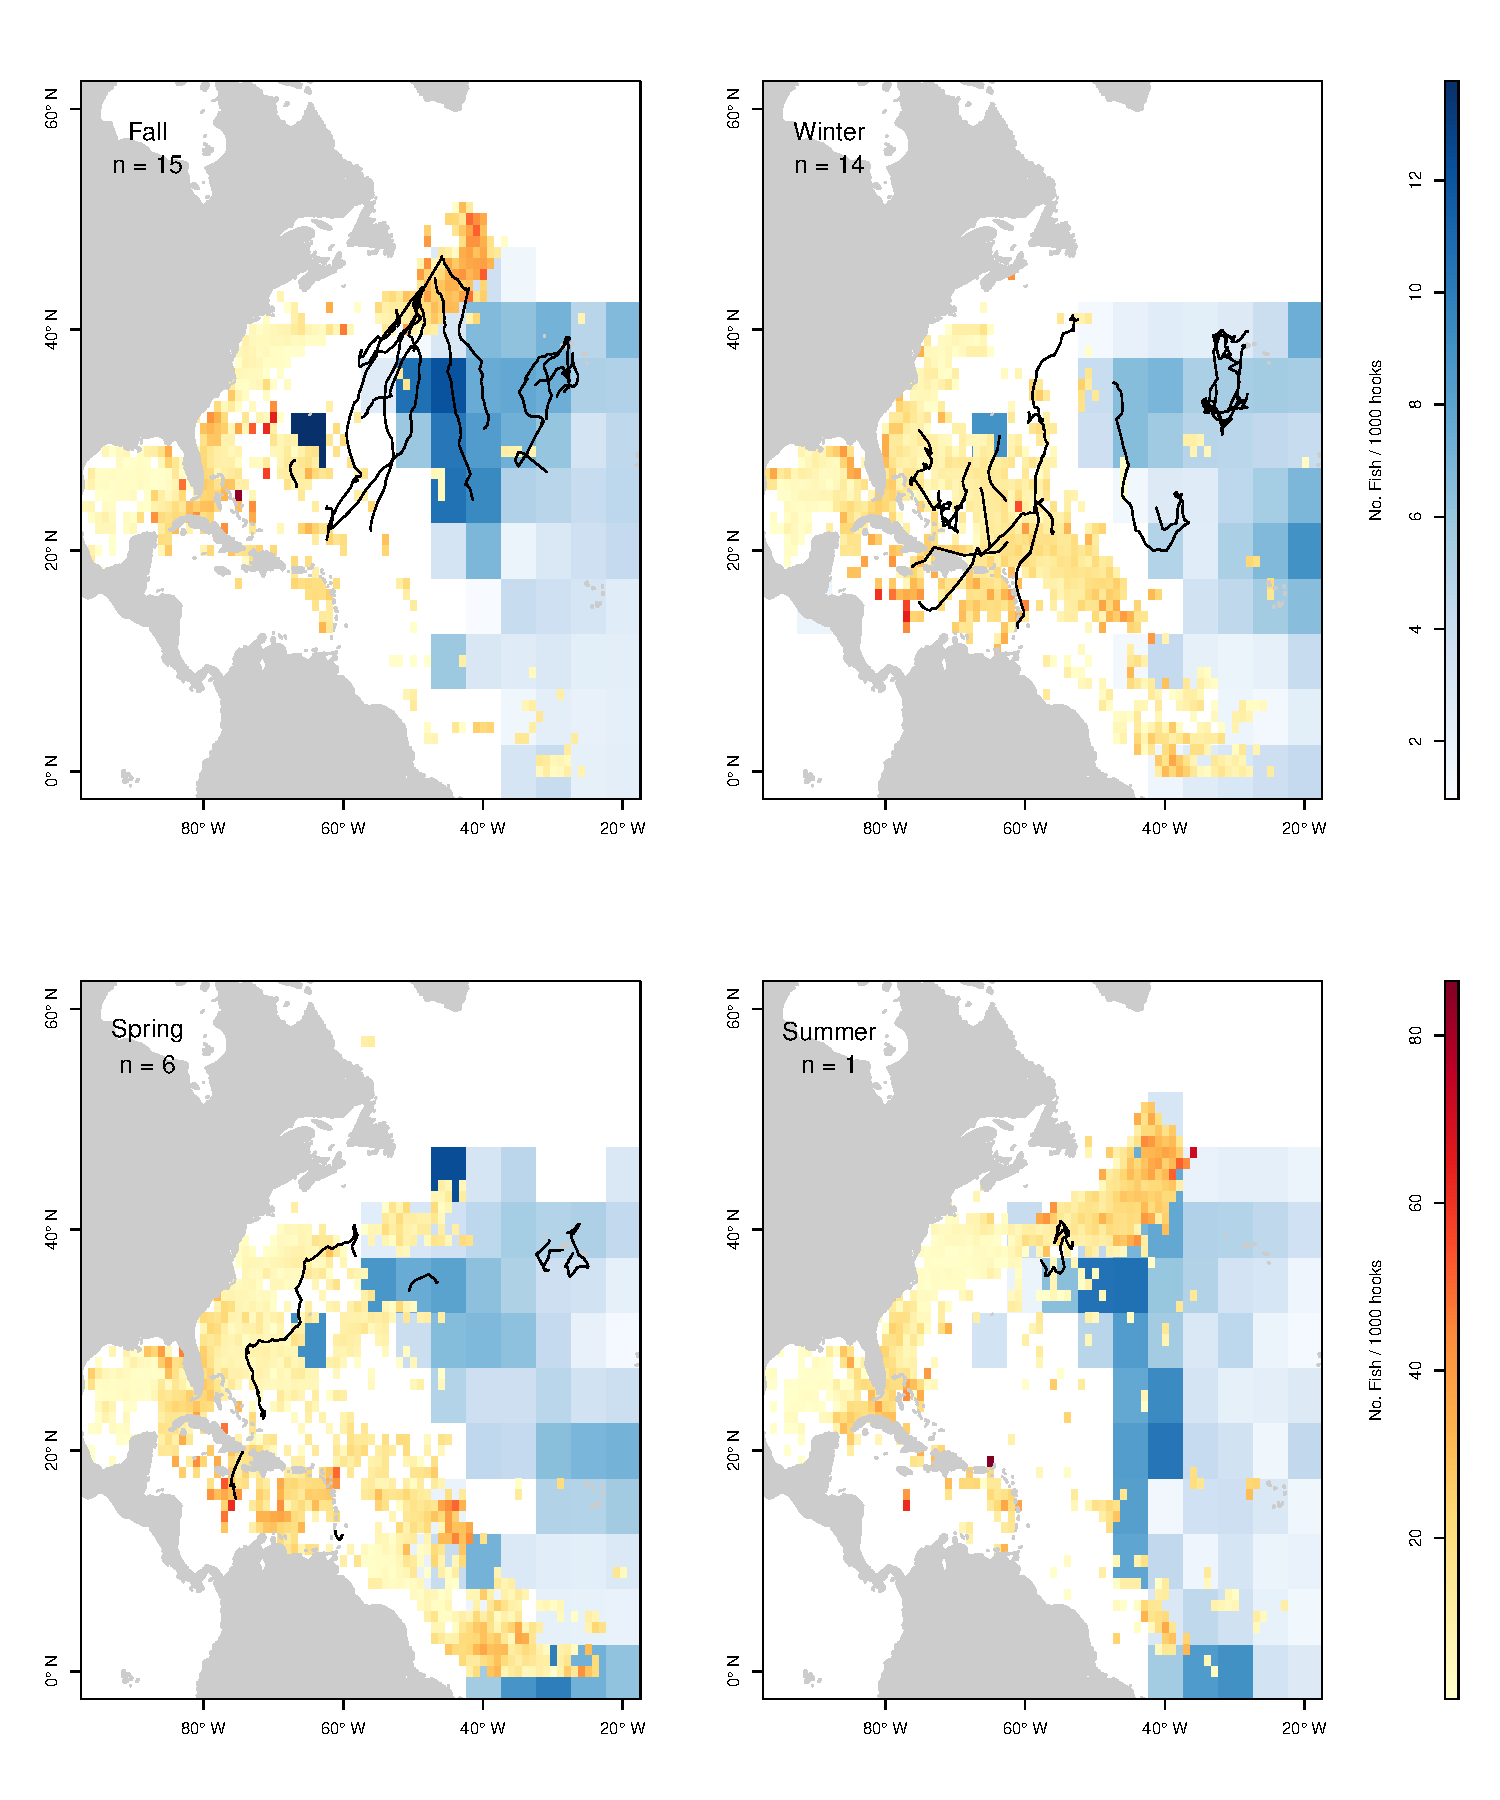
\includegraphics[width=\textwidth]{images/C4_Fig2.pdf}
\caption[Seasonal distribution of catch-per-unit effort of the longline swordfish fishery in the North Atlantic]{Seasonal distribution (Fall: Sep-Nov, Winter: Dec-Feb, Spring: Mar-May, Summer: Jun-Aug) of catch-per-unit effort (number of fish per 1000 hooks) of the longline swordfish fishery in the North Atlantic between 1990-2010 at 5$^{\circ}$x5$^{\circ}$ resolution for the international fleet (blue color scale) and 1$^{\circ}$x1$^{\circ}$ resolution for the U.S. fleet (red/yellow color scale). Tracks of tagged swordfish (this study) shown in black lines (n = number of tagged individuals).}
\label{fig:c4f2}
\end{figure}
%--------------------

\subsection{Oceanographic association}

Swordfish exhibited significant physiological plasticity by occupying a SST range of $\sim$22$^{\circ}$C. Satellite-tagged individuals in the Azores occupied a significantly lower distribution of SST (mean 19.8, range 14.9-28$^{\circ}$C) than either NWA individuals (mean 23.8, range 10.8-28.1$^{\circ}$C; Kruskal-Wallis test, \(p\)<0.001) or conventional tag data (mean 23.3, range 7.2-32$^{\circ}$C; \(p\)<0.001)(Fig. \ref{fig:a4f5}). PSAT-tagged swordfish in the NWA primarily occupied oligotrophic waters with mean chlorophyll values of 0.13 \(mg \cdot m^{-3}\) (range 0.03-1.12). Waters with chlorophyll values above 0.25 \(mg \cdot m^{-3}\) occurred exclusively north of the Gulf Stream or along the southern edge of the Grand Banks. The smaller individuals near the Azores occupied a more restricted chlorophyll range (mean 0.19, range 0.05-0.92 \(mg \cdot m^{-3}\)) but used higher chlorophyll environments more frequently than the adults. Conventional tag data indicated similar affinity for low chlorophyll environments (mean 0.24, range 0.04-7.45 $mg \cdot m^{-3}$) whereby only 2\% of all conventional tag locations with available chlorophyll data were > 1 \(mg \cdot m^{-3}\) (Fig. \ref{fig:a4f5}). Nearly all PSAT-based movements occurred within regions that exhibited ample dissolved oxygen at depth (> 3 \(mL \cdot L^{-1}\) at 500 m); however, the individuals that moved into the eastern Caribbean (n=1) and along the eastern side of the lesser Antilles (n=1) likely experienced DO between 2.5-3 \(mL \cdot L^{-1}\) at 500 m (not shown). The majority of movements from PSAT-tagged fish were relatively directed (\eg less tortuous) through the open ocean but were punctuated by periods of orientation to dynamic topographic features such as shelf break habitats (Fig. \ref{fig:c4f1}). Conventional tagging data was also concentrated around strong bathymetric gradients, particularly along the continental shelf of the eastern U.S. (Fig. \ref{fig:c4f3}), and 45\% of these fish were captured in water <1000 m. We found no significant relationship between fish size and environmental characteristics (SST, bathymetry, chlorophyll) in the conventional tag data using linear regression.

Swordfish in this study were also associated with (sub)mesoscale features across the North Atlantic. Measured SST from the PSAT tags indicated that daily SST ranges regularly spanned 1-3$^{\circ}$C around the Azores and in the Gulf Stream, and ranges >3$^{\circ}$C and as high as 7$^{\circ}$C occured in the front-rich area north of Puerto Rico and in the Azores Front (Fig. \ref{fig:c4f1}). In addition, 69\% of the conventional tag locations (for which remote-sensing data is available; n=8627) occurred in a region of weak front activity (magnitude >0.1$^{\circ}C \cdot km ^{-1}$) while 35\% were in areas characterized by stronger fronts (magnitude >0.5$^{\circ}C \cdot km ^{-1}$). Ten and fifteen percent of conventional tag data occurred on or within 10 km, respectively, of fronts >1$^{\circ}C \cdot km ^{-1}$ in magnitude, which largely occurred along the shelf break of the eastern U.S. from northern Florida to the Grand Banks.

%--------------------
\begin{figure}[htbp]
\centering
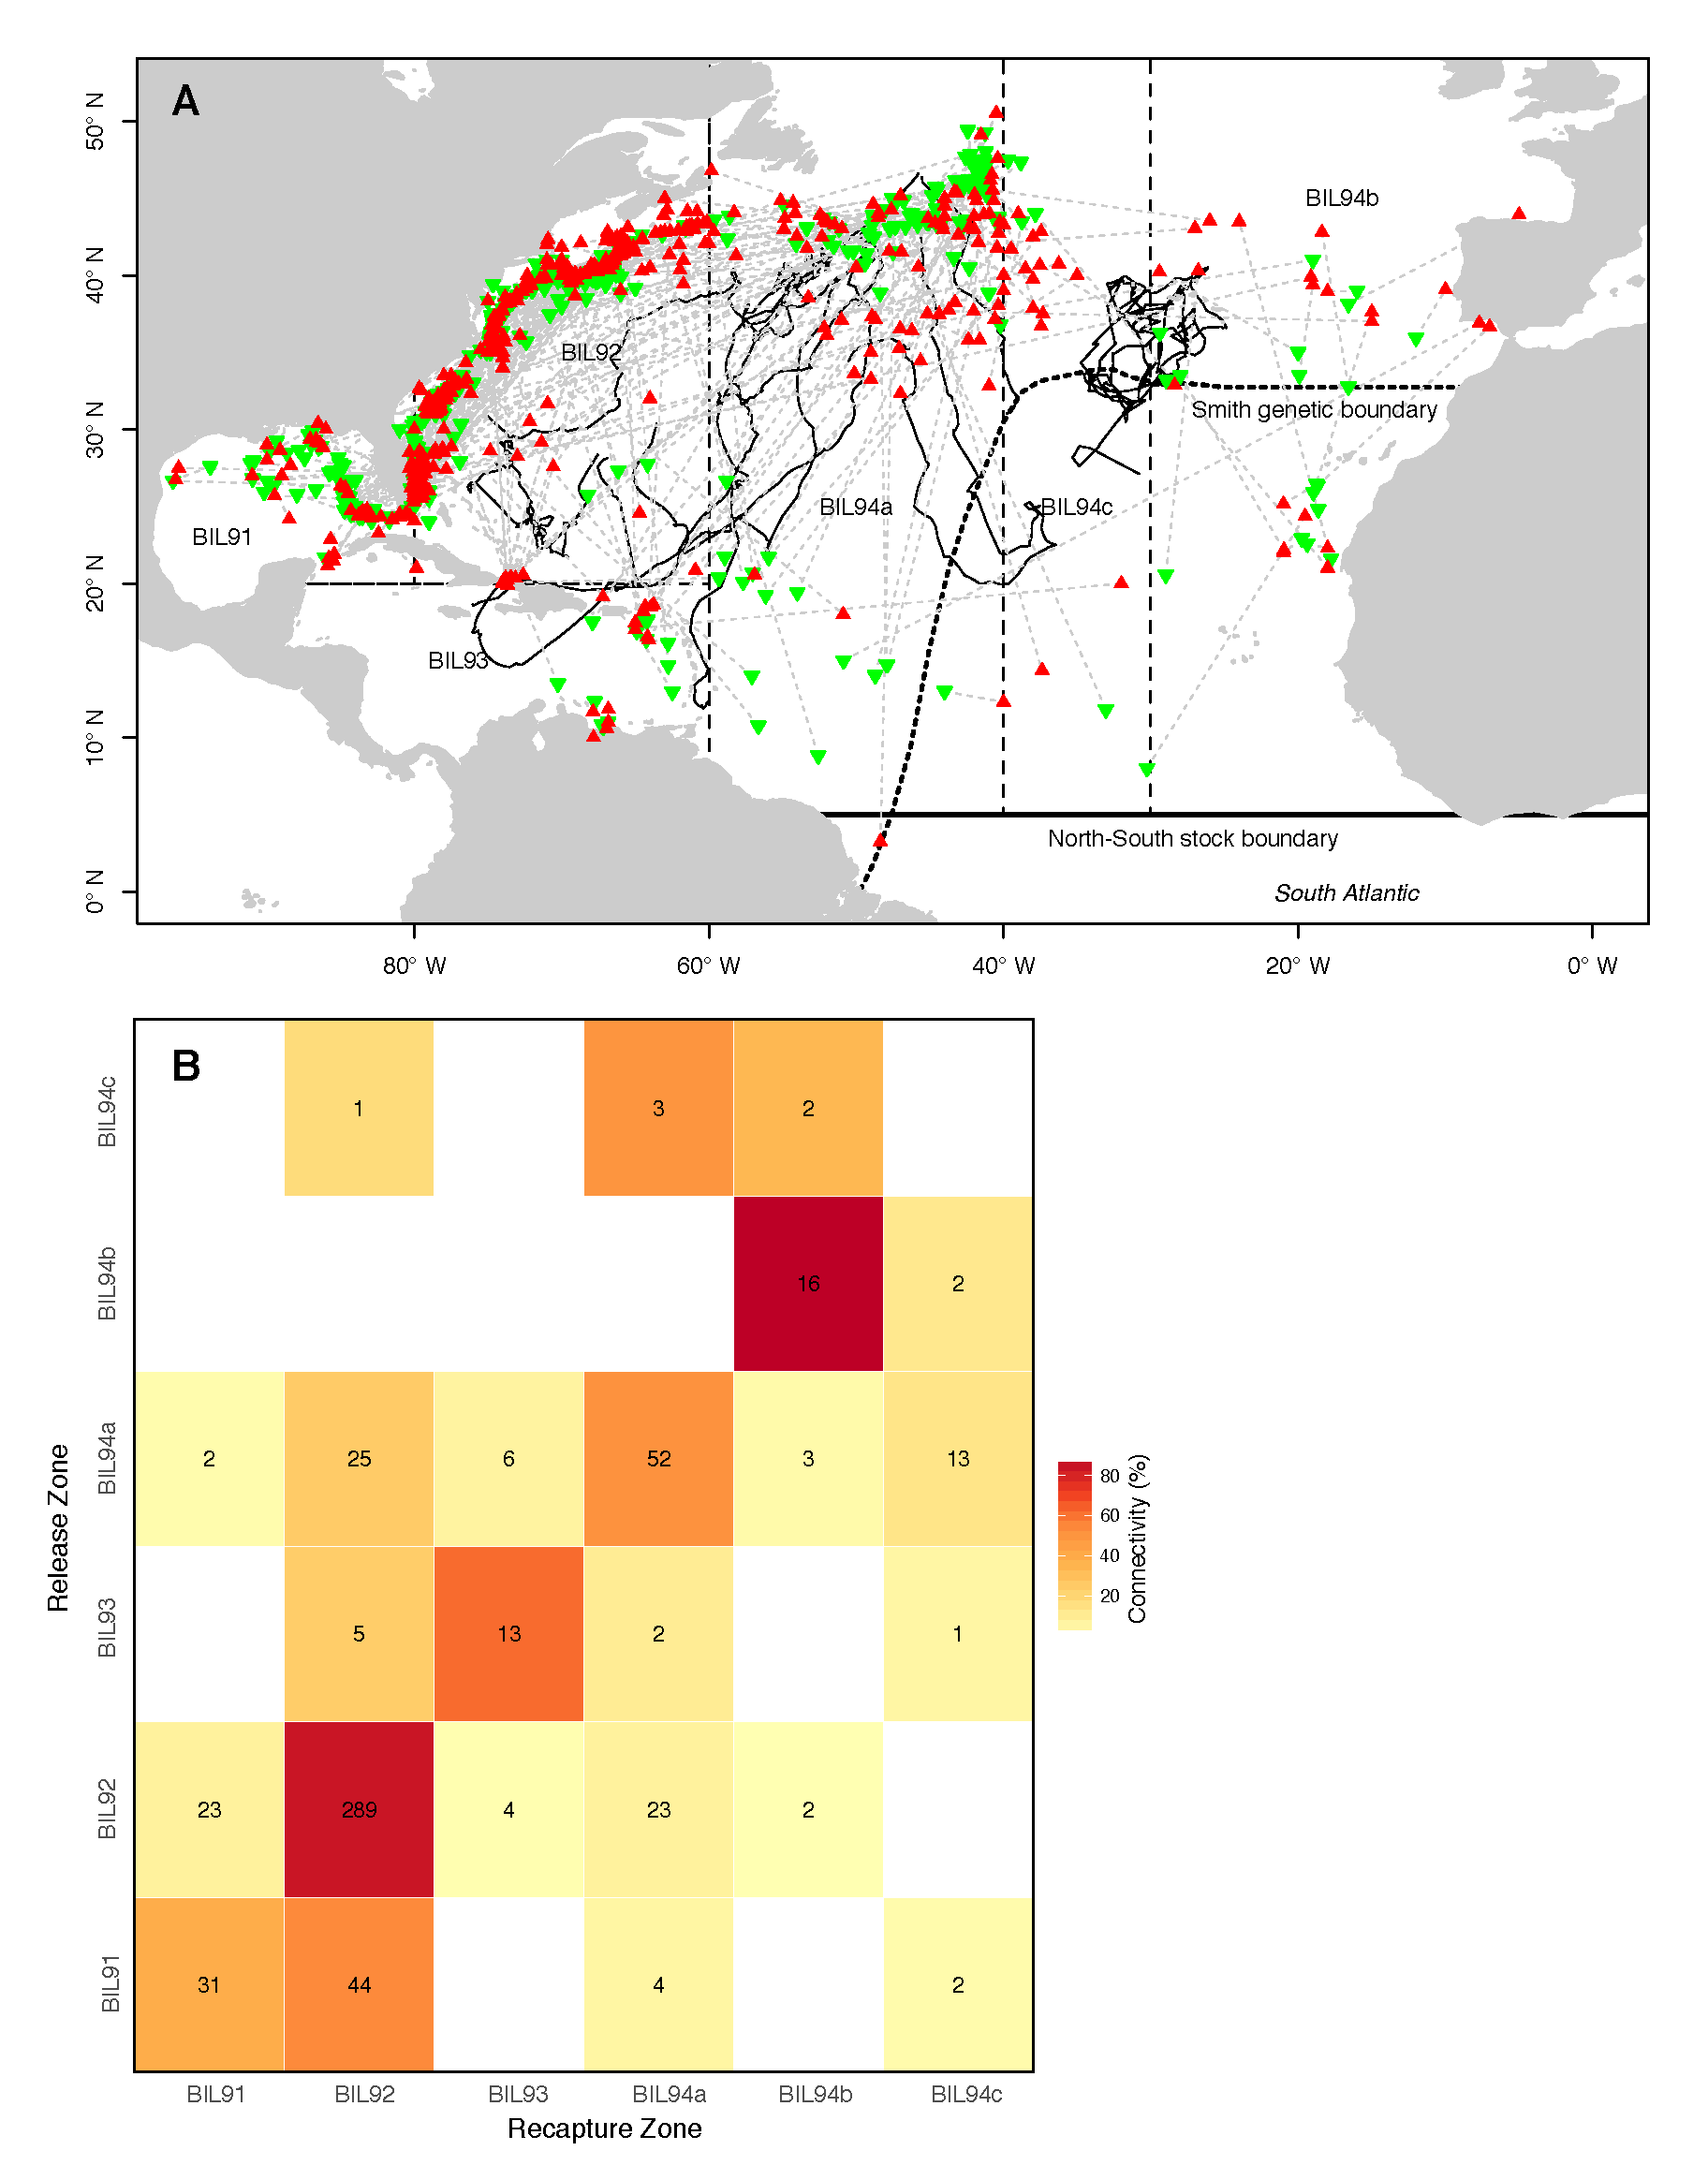
\includegraphics[height=7in, keepaspectratio]{images/C4_Fig3.pdf}
\caption[Movements and connectivity of tagged swordfish in the North Alantic compared to management areas]{Movements (A) of satellite-tagged (black solid lines) and conventional-tagged (dashed grey lines) swordfish in the north Atlantic relative to ICCAT sampling areas (black dashed lines, labeled "BIL9x"). Heavy latitudinal line at 5$^\circ$N indicates north-south stock boundary, and dashed black line from South America to northern Africa is the boundary line from genetic evidence in \citet{Smith2015}. Release (green triangle) and recapture (red triangle) positions of conventional-tagged individuals are shown for recovered individuals. Percent connectivity (B) matrix for release and recapture zones of conventional-tagged swordfish is scaled to total number of releases per zone. Numeric labels indicate relevant number of individuals.}
\label{fig:c4f3}
\end{figure}
%--------------------

While the scale of uncertainty on PSAT track estimates is typically too large to reliably collocate swordfish movements to (sub)mesoscale features \citep[$\sim$100 km;][Chp. \ref{chap:2}]{Braun2018a}, a few PSAT-tagged individuals exhibited tracks and depth-temperature profile data that support their use of eddies. For example, during late March PTT 95975 occupied an open ocean anticyclonic eddy (ACE) offshore from Florida (Fig. \ref{fig:c4f4}A,C) and a cyclonic (CE) Gulf Stream eddy in early May (Fig. \ref{fig:c4f4}B,C). The ACE was characterized by depressed isotherms and warmer water at depth relative to the surrounding Sargasso Sea water (Fig. \ref{fig:c4f4}C). In contrast, the more energetic Gulf Stream CE was >6$^{\circ}$C colder at 400 m than the ambient water and exhibited a core of cool ($\sim$16$^{\circ}$C) water. Using conventional tag data, we were also able to quantify swordfish occupation of eddies in the Gulf of Mexico, Sargasso Sea and the Gulf Stream. In the Sargasso Sea, our data suggested no preference for eddies of either polarity and similar use of within-eddy structure relative to drifters in the same region (Fig. \ref{fig:c4f5}). In the Gulf of Mexico, conventional tags were deployed or recovered within ACEs nearly 70\% more than in cyclones, most of which was focused within ACE cores. The opposite trend was observed for drifters in this same region in which nearly an order of magnitude more drifter locations were in cores of cyclones (Fig. \ref{fig:c4f5}). The Gulf Stream represented the most dynamic region for presence of mesoscale features in the study area. In this region, 2x more swordfish conventional tag locations were found in ACEs than in CEs (Fig. \ref{fig:c4f5}B,E). These data indicate a similar preferential use of the outer cores and inner periphery of ACEs compared to CEs while drifter data in CEs was approximately double that of ACEs.

\subsection{Factors influencing CPUE}

Spatial, temporal and environmental factors were examined for their influence on swordfish catch using GAM analysis. The final model accounted for 46.5\% of the variability in CPUE and included location, month, monthly mean SST, monthly mean SSH, depth of the DSL, mixed-layer depth, distance to the 200m bottom contour and log-transformed chlorophyll as significant predictors (Fig. \ref{fig:c4f6}). Location was identified as the primary predictor of CPUE (explained 37.9\% of variability), followed by SST (3.1\%) and chlorophyll (2\%). The remaining significant predictors each accounted for less than 2\% of the variability in CPUE: MLD, DSL, SSH, month and distance to the 200 m bottom contour. Monthly front frequency and SSH range per cell were both insignificant predictors of CPUE, as was distance to the climatological monthly mean of the north wall of the Gulf Stream.

Based on the GAM smoother functions, catch was highest between 17-23$^{\circ}$C (Fig. \ref{fig:c4f6}A), in low chlorophyll (<0.15 \(mg \cdot m^{-3}\)) environments (Fig. \ref{fig:c4f6}F) and close to the 200 m bottom contour (Fig. \ref{fig:c4f6}E). Catch was also negatively influenced by the most shallow MLDs (< 30 m)(Fig. \ref{fig:c4f6}D) and was higher at mid-range scattering layer depths (350-500 m) than outside that range (Fig. \ref{fig:c4f6}C). The final GAM also found higher catch in areas with high SSH and a similar but weak positive relationship with low SSH (Fig. \ref{fig:c4f6}B).

%--------------------
\begin{figure}[htbp]
\centering
\includegraphics[height=6.75in, keepaspectratio]{images/C4_Fig4.pdf}
\caption[Example use of eddies by an archival-tagged swordfish]{Occupation of an open ocean anticyclonic eddy for 9 days (2011-03-26 to 2011-04-03) (A) and a cyclonic eddy in the Gulf Stream for 5 days (2011-04-29 to 2011-05-01) (B) by a PSAT-tagged swordfish shown in maps of SST (color; A,B) and SSH (contours; A,B). Contours (A,B) indicate negative and positive SSH in dashed and solid lines, respectively, at 5 cm intervals. Dates of the imagery are shown in the top left of map panels (A,B). Upward and downward facing triangles represent entry and exit of the outer contour ($L_s$) of the eddy, respectively, and correspond to dashed vertical lines in the profile plot (C). Note that the satellite imagery used in each panel corresponds to the midpoint in time of each eddy occupation. The bounds of the eddy in the imagery may not correspond to the entry and exit points of the eddy denoted by the triangles as the eddies moved considerably over the period in which the swordfish occupied these features. Depth-temperature profiles from the PSAT tag (C) show a vertical cross section of the occupied eddies (AC=anticylonic, CY=cyclonic). Contours show isotherms at 1$^{\circ}$C intervals.}
\label{fig:c4f4}
\end{figure}
%--------------------

\section{Discussion}

While over 90 archival tags have been deployed on swordfish in the Atlantic \citep{Braun2015}, the oceanographic drivers of swordfish movements remain poorly understood. This is at least partially due to a consistent pattern of diel vertical migration by swordfish that often renders traditional light-based geolocation difficult \citep{Dewar2011, Lerner2013}. Instead, most studies have focused on vertical habitat of swordfish in isolation from the geographic space that the vertical behaviors occurred in due to inadequate light data for reliable geolocation \citep{Abecassis2012, Dewar2011, Evans2014, Loefer2007, Lerner2013}. Here, we employed a recent advance in geolocation analysis methods to supplement missing light data with other forms of data recorded by the satellite tags \citep[][Chapters \ref{chap:2}, \ref{chap:3}]{Braun2018a, Braun2018b}. Depth-temperature profile data on the tags proved particularly valuable for improving geolocation estimates and enabled a more realistic representation of swordfish movements and the oceanographic environments they inhabit.

\subsection{Movements and connectivity}%\label{movements-and-connectivity}

Swordfish in the western North Atlantic exhibit largely North-South movements that are likely driven by contrasting ocean regimes used for feeding and reproduction \citep{Sedberry2001, Abascal2015}. Adults moved from productive foraging grounds in the far north during summer to tropical and subtropical waters in winter to presumably spawn in warm waters that promote larval growth \citep{Arocha1995}. The timing of this migration varied among individuals, but, in general, adults occupied a relatively restricted area within temperate waters from Cape Cod to the Grand Banks during June to October then moved south to a wider region in the (sub)tropics to the Sargasso Sea, Caribbean and Gulf of Mexico from December to March \citep{Neilson2009}. Previous studies have shown a diversity of movements within this general pattern that may be influenced by adult fish homing to spawning habitats \citep{Neilson2009} while smaller individuals exhibit more variability in movements \citep{Abascal2015}. Results from this study corroborated findings of restricted movements among smaller, immature individuals. The movement data from the Azores was comprised entirely of this younger demographic, and these individuals moved between the Azores Front and the Azores archipelago. This may reflect the dominance of foraging needs among immature individuals that changed with ontogeny to larger-scale movements related to spawning. Indeed, mature individuals in this study moved into known spawning areas of the southern Sargasso Sea and Antillean Arc during the spawning period (December through February) \citep{Neilson2013}. However, individuals were typically tagged months earlier and thousands of kilometers away and were not sexed nor was maturity assessed. As such, we are unable to determine the contribution of reproduction to the observed movements.

%--------------------
\begin{figure}[htbp]
\centering
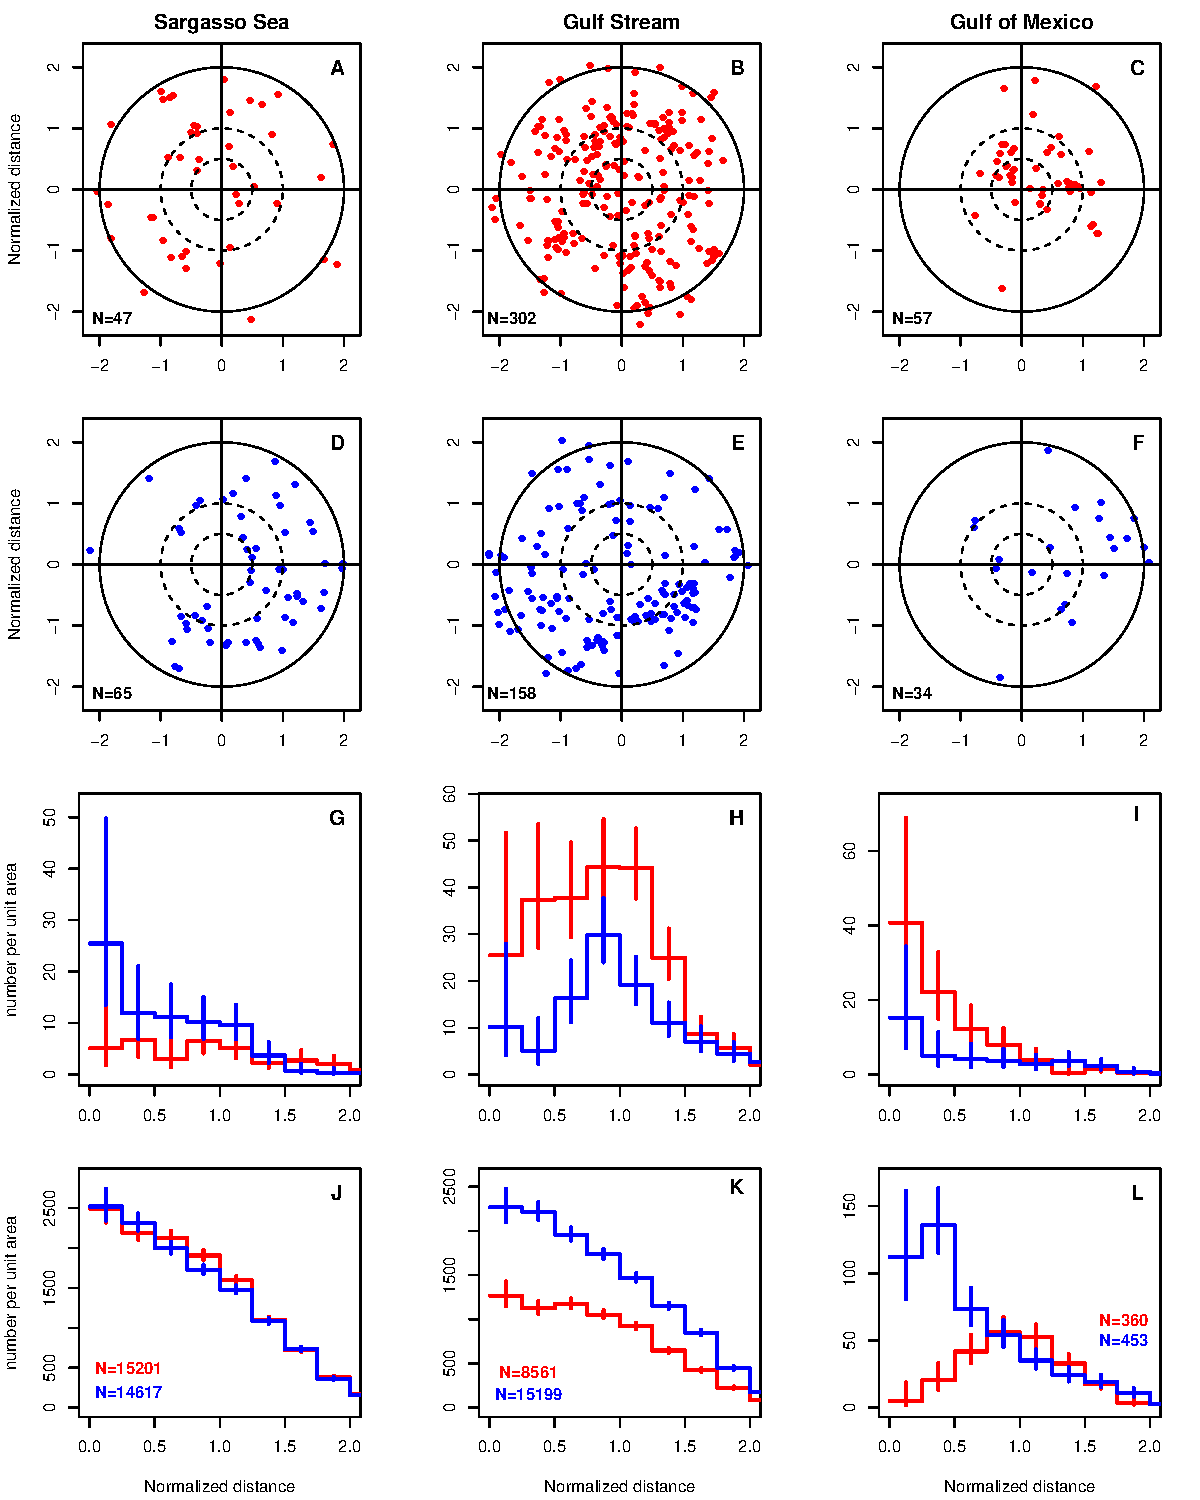
\includegraphics[height=8in, keepaspectratio]{images/C4_Fig5.pdf}
\caption[Collocation of swordfish conventional tag data to anticyclonic and cyclonic eddies across three dynamic regions of the Atlantic]{Collocation of swordfish conventional tag data to anticyclonic (red) and cyclonic (blue) eddies tracked in maps of remotely-sensed SSH across three dynamic regions of the Atlantic: the Gulf of Mexico, the Gulf Stream and the Sargasso Sea. Tag locations were mapped within an eddy-centric reference frame (anticyclones, A-C; cyclones, D-F). Histograms indicate the mean (and 95\% confidence interval, vertical lines) number-per-unit-area of locations within each portion of the eddy-centric frame for swordfish conventional tags (G-I) and drifters (J-L; see methods). Regions and drifter data are shown in Fig. \ref{fig:a4f2}.}
\label{fig:c4f5}
\end{figure}
%--------------------

A recent review of swordfish population connectivity and stock boundaries \citep{Neilson2013} suggested that Atlantic swordfish stocks have recovered from historical overfishing impacts, but complex connectivity patterns complicate stock assessments. Genetic evidence supports separation of North Atlantic, South Atlantic and Mediterranean stocks \citep{Bremer1996, AlvaradoBremer2005a, Smith2015}, and recent work recommended moving the North-South stock boundary as far north as 25$^{\circ}$N east of 45$^{\circ}$W \citep{Smith2015}. However, tagging studies \citep{Abascal2015} suggest a more complex stock structure within the North Atlantic. In our study, no satellite-tagged individuals crossed the current North-South stock boundary at 5$^{\circ}$N, and only one conventional tag deployed near the Grand Banks was recovered across this boundary along the Amazon Delta (Fig. \ref{fig:c4f3}). In contrast, when considering the proposed boundary based on genetic evidence \citep{Smith2015}, 1 PSAT-tagged individual from the NWA, several from the Azores and 11 conventional tag displacements traversed the 50\% probability contour proposed by \citet{Smith2015} based on single nucleotide polymorphism (SNP) analyses. Thus, most tagging evidence supports amended boundaries for stock designation in the Atlantic, but our study suggests a boundary such as that proposed by \citet{Smith2015} may be less effective than the current designation at 5$^{\circ}$N.

\subsection{Oceanographic association}

Ocean dynamics often create barriers to movement, even for highly migratory species, and can have implications from influencing individual behaviors \citep{Stramma2012} to population-level connectivity \citep{Galarza2009, Selkoe2010}. Quantitative analysis of oceanographic association by swordfish has largely been restricted to catch data \citep[\eg][]{Podesta1993} due to the large error inherent in geolocating PSAT-tagged swordfish. Those studies that have investigated oceanographic associations have yielded conflicting results, including association to fronts and bathymetric features in some areas \citep{Sedberry2001} but not in others \citep{Abascal2010}. Here, we improved geolocation estimates from PSAT tag data using depth-temperature profiles and supplemented these results with fisheries data to make robust conclusions about oceanographic association of swordfish in this region.

%--------------------
\begin{figure}[b!]
\centering
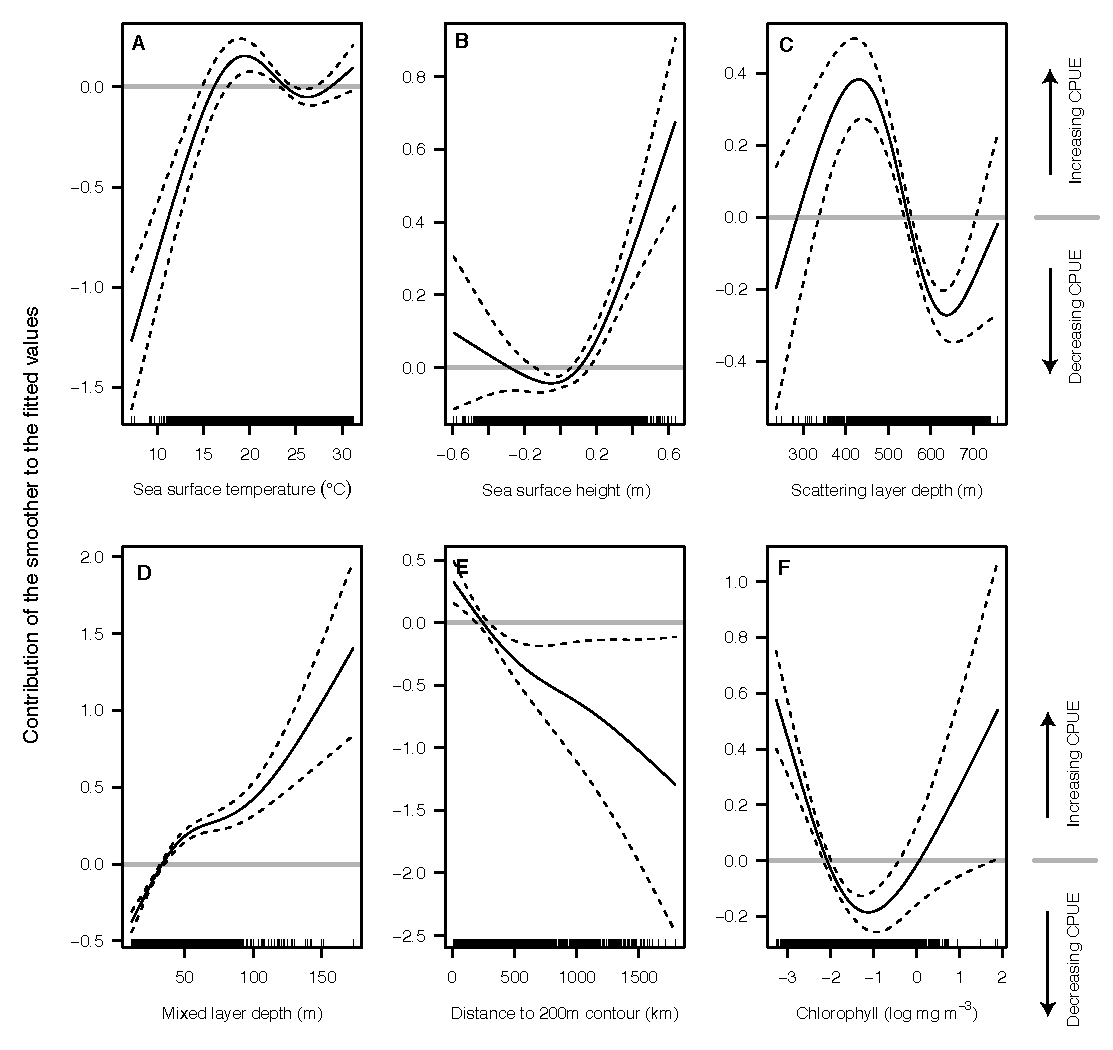
\includegraphics[width=\textwidth]{images/C4_Fig6.pdf}
\caption[Estimated individual effects on swordfish catch per unit effort of environmental covariates in an additive model framework]{Estimated individual effects (solid line) on swordfish catch per unit effort of environmental covariates (A-F). Dashed lines show 95\% confidence limits. Ticks on x-axis indicate values for which data exists. The horizontal line (grey) is added at y=0 to aid visualization. Positive values on y-axis mean higher CPUE.}
\label{fig:c4f6}
\end{figure}
%--------------------

Several tagging studies have reported extreme physiological versatility exhibited by swordfish that are often observed traversing a wide range of SST \citep{Abecassis2012}. This temperature variability is correlated with other biological, physical and chemical oceanographic characteristics, including chlorophyll concentrations and dissolved oxygen concentrations, that are critical for delineating important habitat for swordfish. For example, \citet{Seki2002} characterized the oceanographic regime on swordfish longline fishing grounds in the subtropical Pacific as highly dynamic (as determined primarily by temperature data) with relatively low chlorophyll (<0.4 \(mg \cdot m^{-3}\)). The dynamic nature of swordfish habitat is consistent across ocean basins \citep{Hazin2008, Seki2002, Podesta1993}, as is frequent occupation of SSTs $\sim$20-22$^{\circ}$C \citep{Santos2006}, with reproduction occurring in warmer waters >22$^{\circ}$C \citep{Palko1981, Romeo2011}. Yet many individuals, particularly adults, are regularly observed in temperate waters characterized by cooler SST <20$^{\circ}$C \citep{Evans2014, Abascal2015}, presumably to forage. While DO has been shown to restrict movements in swordfish and other billfish \citep{Stramma2012, Braun2015}, it is unlikely to be a major driver of movements in the temperate and subtropical Atlantic. Nearly all PSAT-tagged swordfish in our study transited ambient DO >3 \(mL \cdot L^{-1}\), even at depth.

The dynamic oceanographic environments preferred by swordfish are also apparent in their proximity to complex topographic features, such as shelf break habitats, submarine canyons and seamounts, that were frequented by tagged fish \citep{Podesta1993, Neilson2009, Palko1981} and have been shown to positively influence swordfish abundance \citep{Hazin2008, Bigelow1999, Scales2017}. Additional inference from our GAM analysis of CPUE data suggested higher abundance of swordfish at intermediate (350-500 m) scattering layer depths and deeper mixed layers (>50 m). The correlation between swordfish CPUE and scattering layer depth may be a product of accessibility of DSL organisms to swordfish. Foraging opportunities for swordfish may increase as the surface mixed layer deepens and DSL shallows in a manner consistent with previous studies on scattering organisms in the Atlantic \citep{Marchal1993}. Our MLD results roughly corroborate findings by \citet{Scales2017} in that both found MLD >30 m had a positive influence on swordfish catch. However, \citet{Scales2017} also found a decreasing probability of the presence of swordfish with MLDs deeper than 90 m based on observer data from the California drift gillnet fishery with spatial and temporal resolution of 0.1$^{\circ}$ and 1 day, respectively, that we did not observe in our data. It is possible that the difference in catch rates with depth between the eastern Pacific and NWA are a function of stronger coupling between upwelling in the California Current system and swordfish behavior. However, we would note that there were also significant differences in spatial and temporal resolution between the studies that made direct comparison of results difficult.

\subsubsection{Thermal fronts}

Fronts often play a key role in marine ecosystems as they delineate water mass boundaries and can elicit dramatic changes in marine biota \citep{bakun2006fronts}. These features are typically associated with convergence zones that aggregate particles, including lower trophic level organisms \citep{Olson1985}, making them particularly attractive foraging areas for a range of marine species \citep{Bost2009, Polovina2000, Scales2015, Teo2007, Miller2015, Queiroz2016}. In our study, association with thermal fronts north of $\sim$25$^{\circ}$N in the NWA is most likely due to enhanced foraging opportunities during the productive northern summer. Based on stomach contents surveys \citep{Stillwell1985}, cephalopods are the predominant component of swordfish diet during this time period along the shelf break from Cape Hatteras to the Grand Banks, and this region is characterized by complex thermal fronts which have been shown to aggregate one of the swordfish's primary forage species, shortfin squid (\emph{Illex illecebrosus})\citep{Wilk1988}. Further south, the use of fronts is typically associated with spawning as these dynamic habitats may aggregate larvae and early juveniles at forage rich frontal zones \citep{Rooker2012, Suca2017} and may increase advection toward foraging grounds in the northwest Atlantic by the Gulf Stream \citep{Olson1994}.

\textit{In situ} SST from the PSAT-tagged individuals in the Azores demonstrated consistent daily SST ranges > 1$^\circ$C, suggesting use of front habitats in this region (including the persistent Azores Front). The Azores Front has been shown to effectively capture and aggregate incoming particles \citep{Sala2016}, potentially generating enhanced foraging opportunities \citep{Olson1985} for rapidly-growing juvenile swordfish. If higher forage densities are indeed associated with thermal front boundaries, the regular presence of fronts along, for example, shelf break habitats may provide a predictable feeding location and thus consistent swordfish catch and effort. This seems to be particularly true along the shelf break of the eastern U.S., where previous studies found 80\% of longline fishing effort to be within 40 km of surface thermal fronts \citep{Podesta1993}, further supporting the conclusions from conventional and satellite tags in this study.

\subsubsection{Mesoscale eddies}

Mesoscale eddies have been identified as "hot spots" of biological activity from primary producers \citep{McGillicuddy2007} to large pelagic fishes \citep{Hobday2014, Gaube2018}. Some evidence suggests eddies create preferred habitats for many large pelagic predators including yellowfin and bluefin tuna \citep{Teo2007, Hsu2015}, white sharks \citep{Gaube2018}, marine mammals \citep{Bailleul2010} and seabirds \citep{TewKai2009}. While divergent trends between swords and other predators have been found on NWA feeding grounds in which swordfish were more often found outside of eddies than within them \citep{Hsu2015}, our results corroborate additional findings by \citet{Hsu2015} which suggest that within eddies swordfish prefer ACEs over CEs in the Gulf Stream region, which has also been shown in the California Current \citep{Scales2017}. Conventionally tagged swordfish in our study were caught more often in ACEs than CEs in the Gulf Stream region, suggesting a preference for ACEs by the integration of individual swordfish behavior and fishing effort measured by conventional tags. A similar pattern was observed in the Gulf of Mexico despite a significantly reduced sample size. Conventional tag data in the Sargasso Sea suggested higher occupation of cyclones, perhaps due to warm water at depth regardless of eddy polarity and the relatively higher productivity in cyclones \citep{Gaube2014} in this region \citep[except see ][]{Dufois2016}. We cannot tease apart these interacting effects of fish ecology and fisher behavior from our data. However, ACEs in the Gulf Stream region are characterized by high temperature anomalies at depth which may make their deep scattering layer prey more accessible in these environments as thermal constraints may be alleviated \citep{Gaube2018}. In addition, while ACEs are predominantly characterized by low surface chlorophyll \citep{Gaube2014}, they can also exhibit high surface chlorophyll, particularly in subtropical gyres \citep{Dufois2016}, and have been recorded containing anomalously high biomass at depth \citep{Fennell2015}. Conventional and satellite-tagged swordfish also occupied CEs, suggesting that their versatile physiology allows them to exploit DSL organisms even in low-temperature environments at depth. The results of the eddy collocation in this study were further supported, at least for ACEs, by the GAM analysis of catch data. This provides additional evidence for swordfish occurrence in high SSH environments (ACEs) across the North Atlantic.

Future investigations of swordfish occupation of eddies, particularly using conventional tag data, should seek to control for the effect of fishing effort on these results. An additional "control" experiment could be added to determine the influence of eddy population in each region. For example, the Loop Current in the Gulf of Mexico only generates anticyclones which may drive significantly different eddy use dynamics by pelagic predators in this region relative to regions such as the Gulf Stream with approximately equivalent generation of eddies of each polarity.

\section{Conclusions}

While swordfish stocks have likely recovered from overfishing in the Atlantic basin, several outstanding questions hinder more robust stock assessment and improved understanding of species' response to climate change. We analyzed the results of a fisheries-independent electronic tagging program in the context of fisheries data. Our approach facilitated inference from decades of data-rich, but summarized, fishery records and independent, high-resolution tag data. Together, these datasets suggest limited connectivity between North and South Atlantic stocks, but we also found little exchange between the northeast and northwest Atlantic. Despite these apparent barriers, swordfish are clearly able to traverse dramatically different oceanographic regimes that may help this species adapt to a changing ocean. Swordfish in our study clearly frequented (sub)mesoscale features throughout their range; however, improvements in tag technology and associated error will be required to more adequately characterize the relationship and relative importance of fronts and eddies for swordfish in the NWA and beyond.
